\chapter{Methodologies}
\graphicspath{{Chapter3/Figs/}{Chapter3/Figs/}}

This chapter describes the project-related academic methodology and the planned approach. The reader is introduced to the rationale for the intended workflows, hardware, and software tools.

\section{Background}
\label{chapter3-background}

A methodology used to conduct research in order to build a N/CI with the assumed requirements as describe with the three-dimensionality was to do a case study at the research and development (R\&D) team at IDUN Technologies. IDUN Technologies had in the end of 2021 a PoC of a closed loop system of their Neuro-Intelligence Platform (NIP), which is a term they use for marketing to give their N/CI a trademark-ready name as depicted on \autoref{fig:idun-nip}. The PoC consisted of a web-based single-page application (SPA) hosted on AWS Amplify, which is a backend-as-a-service from the AWS cloud that simplifies the deployment of SPAs connecting it to a GraphQL API via the AWS AppSync.

\begin{figure}[!ht]
  \centering
  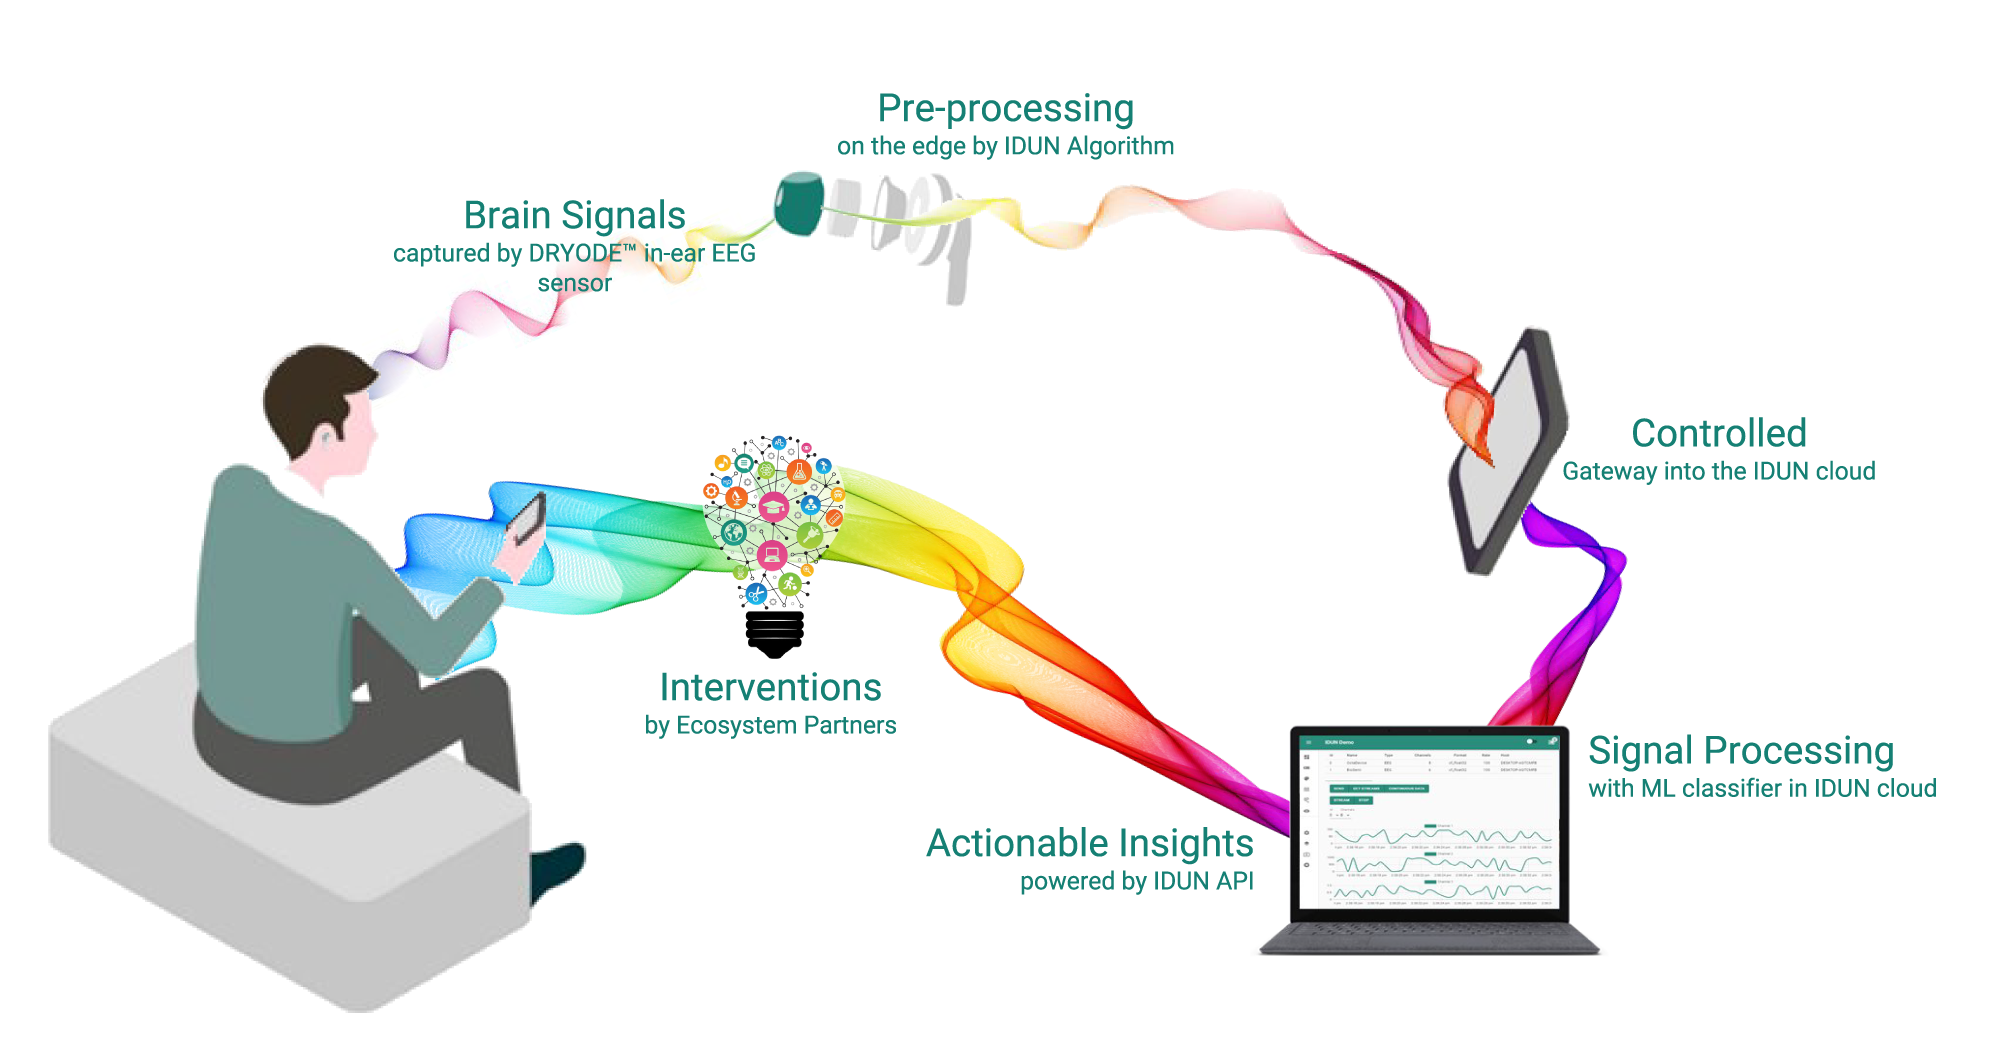
\includegraphics[width=\linewidth]{idun-nip.png}
  \caption{IDUN Technologies' representation of their N/CI, which they refer to as a closed neurofeedback loop or, for marketing purposes, "Neuro-Intelligence Platform" (NIP) (IDUN Technologies, 2022).}
  \label{fig:idun-nip}
\end{figure}

\section{Case study}
\label{chapter3-case-study}

% Forty-three patients of the psychiatric clinic with diagnosed major depression (12 male, Mage = 36.35, SDage = 7.92) participated in this study for monetary compensation (10 USD).

\section{Procedure}
\label{chapter3-procedure}

\subsection{Project stages}
\label{chapter3-project-stages}

% - The study used a between-subject design (treatment group, control group) with the
% depression score on the XXX depression scale as dependent variable.
% - The study used a within-subject design (pre-treatment measurement, post-treatment
% measurement) with the depression score on the XXX depression scale as dependent variable.
% - The study used a mixed design with the between-subject factor group (treatment, control) and the within-subject factor time (pre-treatment, post-treatment). The depression score on the XXX depression scale served as the dependent variable.

% - Three types of materials were used. First,… Second,… Third,…

% - Before the experiment started, participants were randomly assigned to two groups: the X group and the Y group.
% - The experiment consistent of two phases. In the first phase,….. . In the second phase,…. .
% - The order of these two phases was counterbalanced
% - First, participants had to… next… subsequently… finally…
% - Simultaneously,…
% - After participants finished X, they… % Example citation

\subsection{Group discussions}
\label{chapter3-group-discussions}

\subsection{Expert interviews}
\label{chapter3-expert-interviews}

\section{Outcomes}
\label{chapter3-outcomes}

\section{Reflection}
\label{chapter3-reflection}

\section{Further development}
\label{chapter3-further-development}

% - First, they were randomly assigned to treatment and placebo group
% - Both groups: 60 minutes intervention
% - Treatment group: first,… next,…
% - Placebo group: first, …next,…
% - Finally, they filled out the depression questionnaire
% o Did you describe everything that is needed to replicate your research?
% o Did you cite the sources of your methods or paradigms?

\nomenclature[rd]{R\&D}{Research and development}
\nomenclature[nip]{NIP}{Neuro-Intelligence Platform}
\nomenclature[spa]{SPA}{Single-page application}